\section{Motivation and related work}
\label{sec:motive}

Setting an invocation latency goal in the 10s of $\mu{}s$ based on the network
requires \textit{even lower} local invocation latencies on the compute node.  To
determine whether the design of traditional containerized FaaS systems is compatible
with this goal, we establish a lower bound on the latency achievable using
containers:\ we remove the containers altogether and model each microservice as a
separate process.  In this model, a cold start translates to a
\texttt{fork()/exec()}.  The large number of microservice processes means that our
warm start story cannot involve their remaining scheduled.  As such, we cause
inactive tasks to block and later wake them up with a Unix IPC mechanism; the
latencies of the available mechanisms being similar [\solb{CITE}], we opt for loopback UDP.
These two variants are shown in Figure~\ref{fig:motive} as the blue and green lines,
respectively.  Unfortunately, even the average warm start latency is high enough to
soon become a bottleneck on datacenter networks; worse, the 99.9\% tail latency
exceeds 10 $\mu{}s$, already slower than a network RPC.

From this we decide to eschew the separate processes for each microservice.  Instead,
we propose collecting groups of microservices into shared \textbf{worker processes},
each responsible for performing all the work assigned to a given CPU core.  We can
assume that these will always be running, so the cold start case now only requires us
to load user code into an existing process.  We do this by packaging user
microservices as shared object files and using the dynamic linker/loader's
\texttt{dlopen()} interface.  Because each worker owns its cores, they can spend any
(rare) time between user tasks polling for the next job to arrive, so a warm start
simply involves flipping a ready bit in memory shared between the two processes.
Both cases appear in Figure~\ref{fig:motive} as the orange and red lines,
respectively.  This time, the warm start is significantly faster than our objective
at just a few hundred \textit{nanoseconds}, with the 99.9\% tail below 2 $\mu{}s$.

\begin{figure}
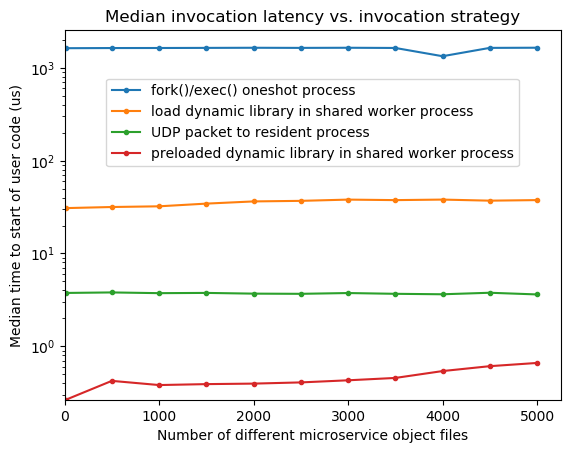
\includegraphics[width=\columnwidth]{figs/2018-02-02-motivation_numfuns-latency-reordered}
\caption{Median one-way invocation latencies for a microservice that does no work (note the log scale)}
\label{fig:motive}
\end{figure}

We conducted this benchmark and all other experiments on one 16-core socket of a
Linux 4.13.0 equipped with 2.1-GHz Xeon E5-2683 Broadwell processors.  One physical
core was dedicated to a host-wide \textit{dispatch process} that spools requests and
forwards them to 14 physical cores dedicated to running the microservices; the
remaining core was reserved for use by a thread that would communicate with the wider
serverless cluster management system.

We would be remiss to suggest consolidating multiple users' jobs into a single
process without addressing the security implications of doing so.  Clearly, we must
somehow replace the isolation we are sacrificing with this design choice; meanwhile,
we must remember that we made the choice to meet extreme performance objectives, and
avoid adding protections that incur significant runtime cost.

Fortunately, we can learn from two recently-published systems whose own extreme
performance requirements drove them to perform similar coalescing of traditionally
independent components:  NetBricks~\cite{Panda2016} is a network functions runtime
for providing enhanced network capabilities; it is unique among this class of
systems for running the submitted functions in-process rather than in VMs.
Tock~\cite{Levy2017} is an embedded operating system that provides (in addition to a
more traditional process model) a type of lightweight application known as a capsule
that is embedded within the kernel and communicates with it using simple function
calls.  As their primary line of defense against untrusted code, both systems
leverage Rust~\cite{www-rustlang}, a new type-safe systems programming language.

Rust is a strongly typed, compiled language that reprises C's abstention from a
heavyweight runtime.  Unlike many other modern systems languages, Rust is an
attractive choice when both performance and predictability are critical due to its
lack of a garbage collector.  Still, it manages to provide strong memory safety
guarantees by focusing on ``zero-cost abstractions'' (i.e., compile-time checks).  In
particular, safe Rust code is guaranteed to be free of null or dangling pointer
dereferences, invalid variable values (e.g., casts are checked and unions are
tagged), reads from uninitialized memory, mutations of non-\texttt{mut} data (roughly
the equivalent of C's \texttt{const}), and data races, among other
misbehaviors~\cite{www-rustlang-ub}.

We require each microservice to be written in Rust, which gives us many aspects of
the isolation we need:  It's difficult for microservices to crash the worker process,
since most segmentation faults are prevented, and runtime errors such as integer
overflow generate Rust panics that we can catch.  They can't get references to data
that doesn't belong to them because of the data and pointer initialization rules.
However, given our performance goals, there is a significant aspect of isolation that
Rust doesn't provide:\ there is nothing to stop users from monopolizing the CPU.
While it is true that other modern systems languages such as Go~\cite{www-golang} and
Erlang~\cite{www-erlang} include so-called ``green threading'' (support for sharing a
kernel thread among multiple tasks), this multitasking is implemented cooperatively,
so a task in a tight loop will never yield.  To prevent this kind of behavior, our
system needs to be preemptive.

The reader may be suspicious at the suggestion that we need to implement preemption,
given that operating systems have provided this functionality as a core service for
close to half a century.  However, we emphasize that our goals differ significantly
from those of an operating system:  An OS kernel avoids frequent preemption due to
the significant cost of rescheduling preempted work.  In contrast, the microservices
in our model are unapologetically lightweight and short-lived, and our system can
just kill any that time out.  Enforcing hard time limits is already an established
attribute of serverless systems, with the three large providers already limiting
microservices to minutes of runtime; we merely propose significantly reducing this
time budget.

Of course, the question remains of how to achieve preemption.  We initially doubted
the existence of any efficient mechanism for truly fine-grained preemption; however,
upon benchmarking the capabilities of the POSIX \texttt{setitimer()} interface, we
were surprised to find that modern CPUs' HPETs (high precision event timers) permit
reliably signaling a process as often as every few microseconds, and this approach
scales to operating on all cores simultaneously.
